\section{Porting Challenges}

Although the pre-Exascale machines gave the VTK-m development team good experience porting to different processor architectures, the design of the Exascale machines Frontier and Aurora introduced new technical challenges.
This section reports the most major modifications of VTK-m to make it feasible to run on the Exascale hardware.

\ken{
  Each subsection should be roughly 1/3 page.
  (1 + 1/3 page total.)
  The subsection should start with a paragraph defining the problem/motivation.
  The following paragraph should give an overview of the approach.
  The remaining paragraphs can go into technical challenges that were encountered and how they were addressed.
}

\subsection{Adopting Kokkos}

\assign{Sujin}

\begin{figure}[htb]
  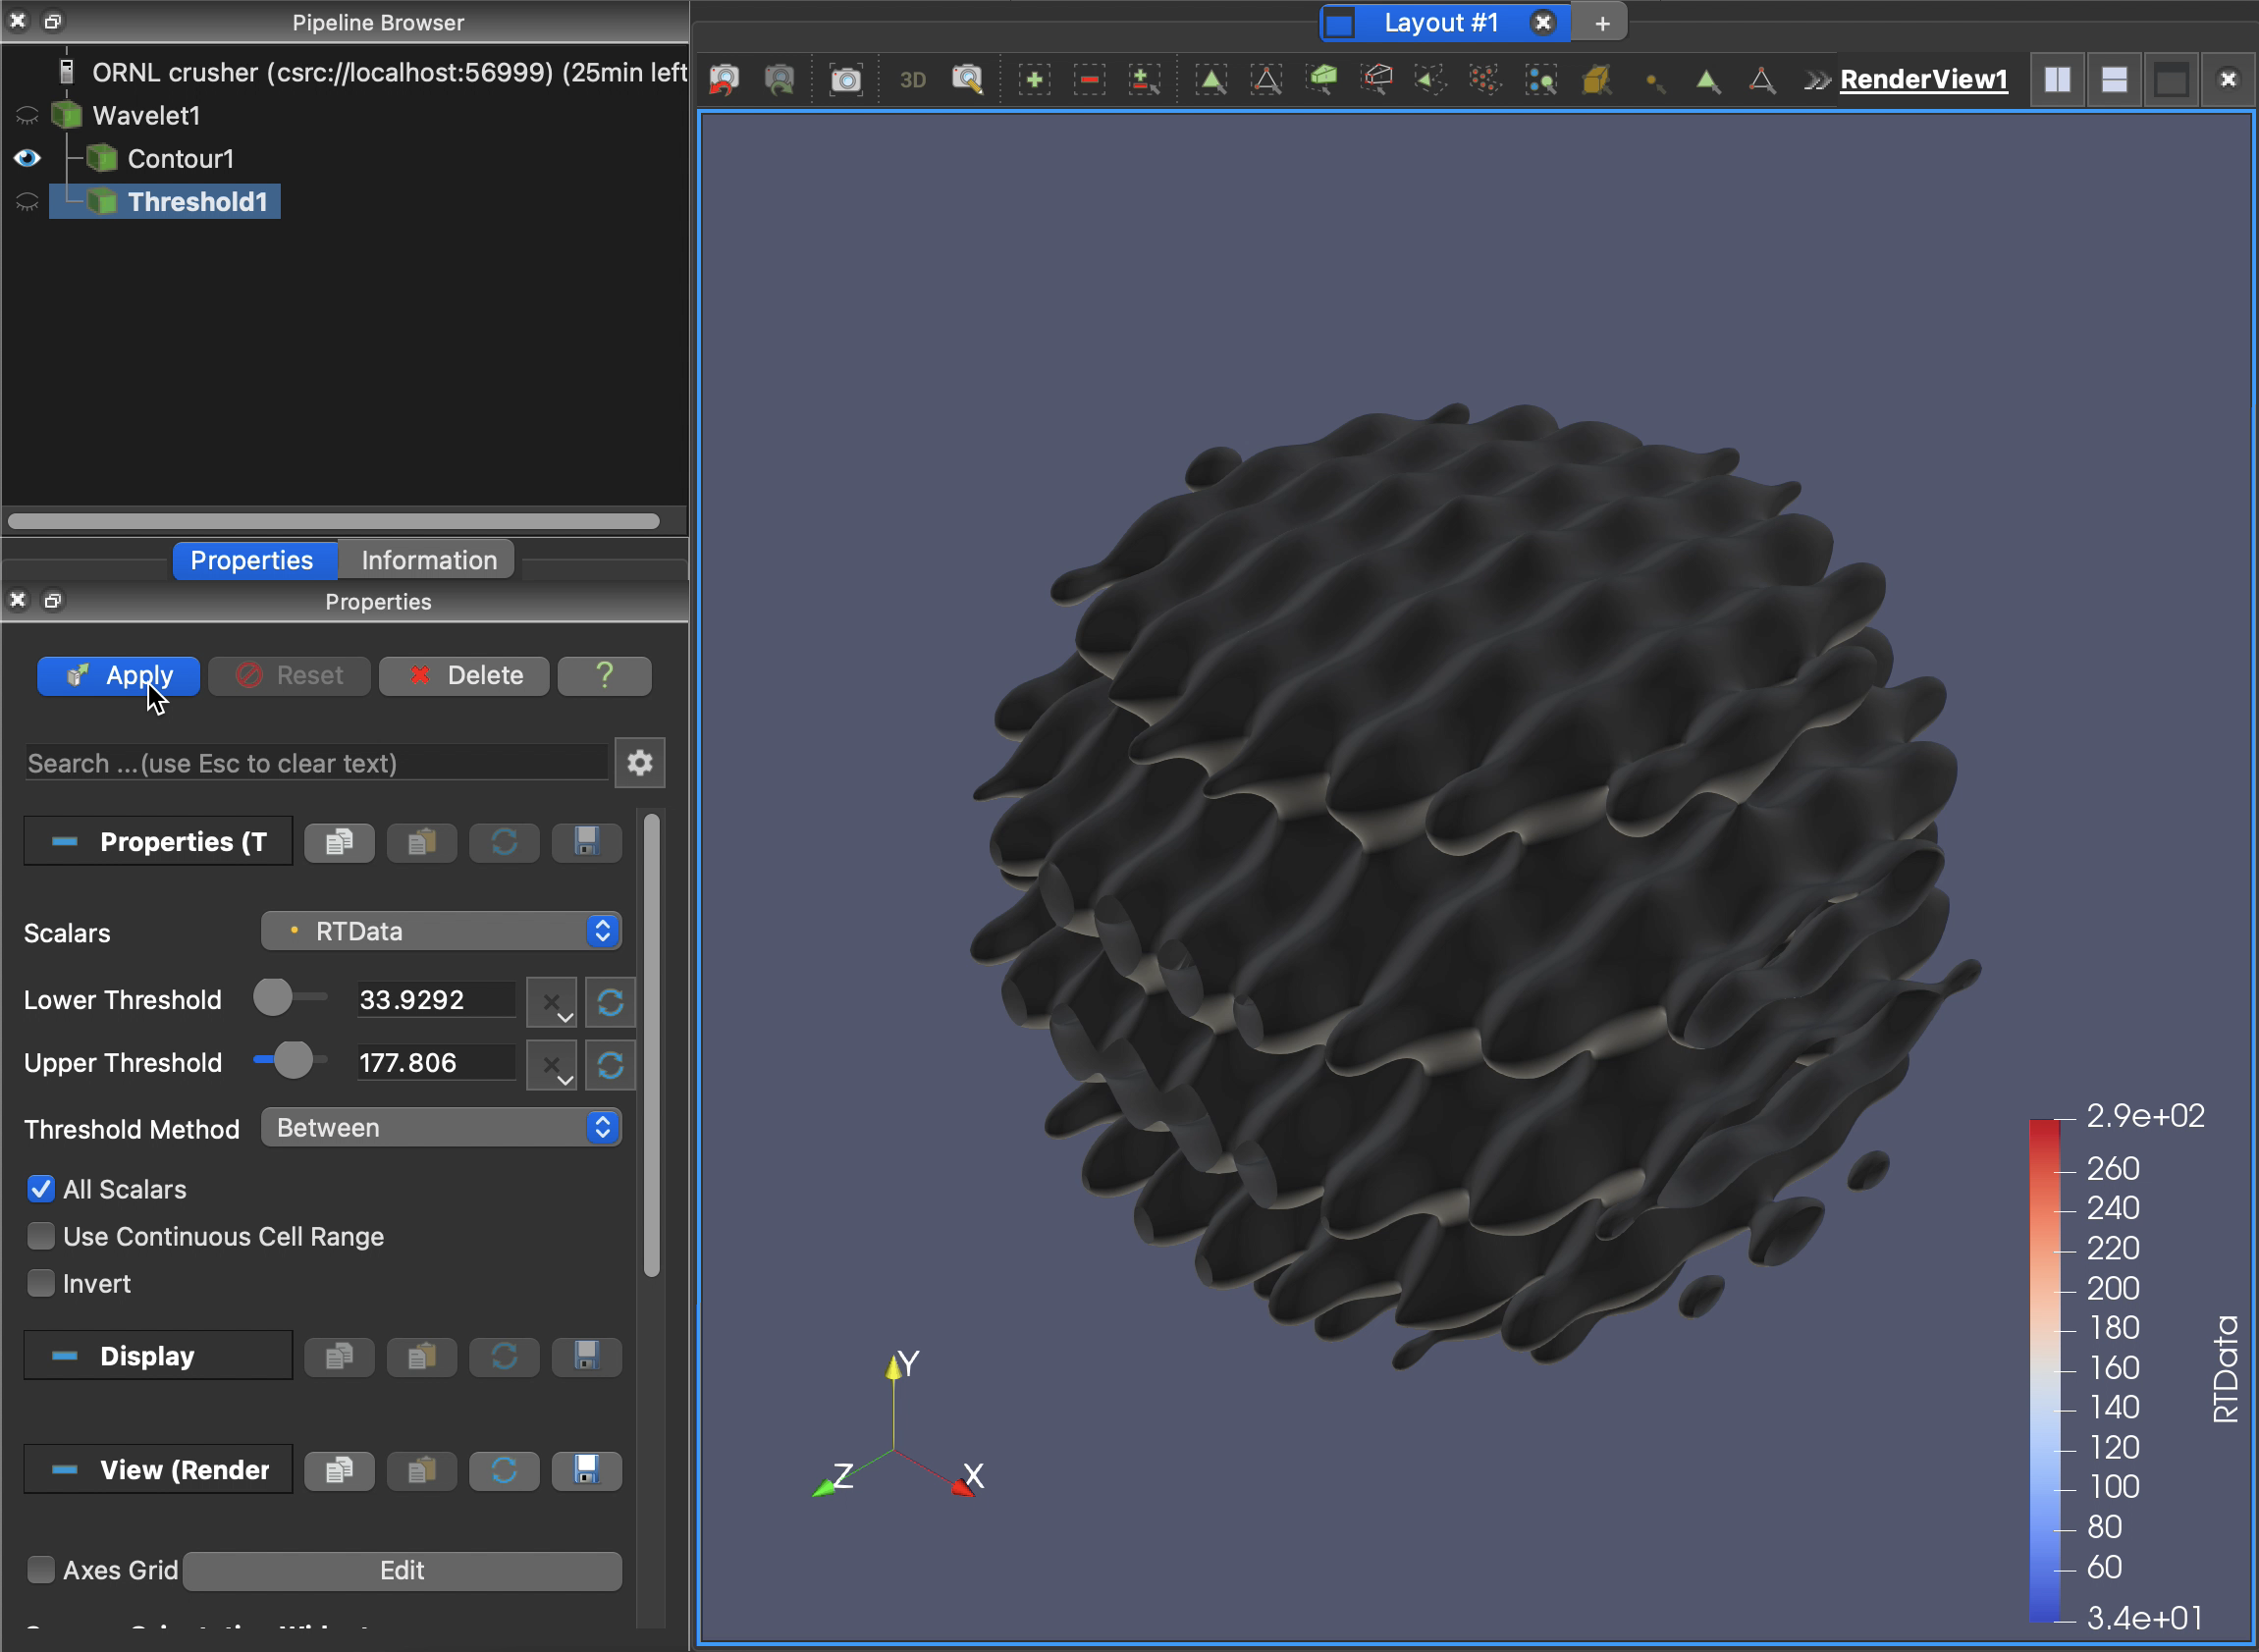
\includegraphics[width=\linewidth]{figures/paraview-crusher.png}
  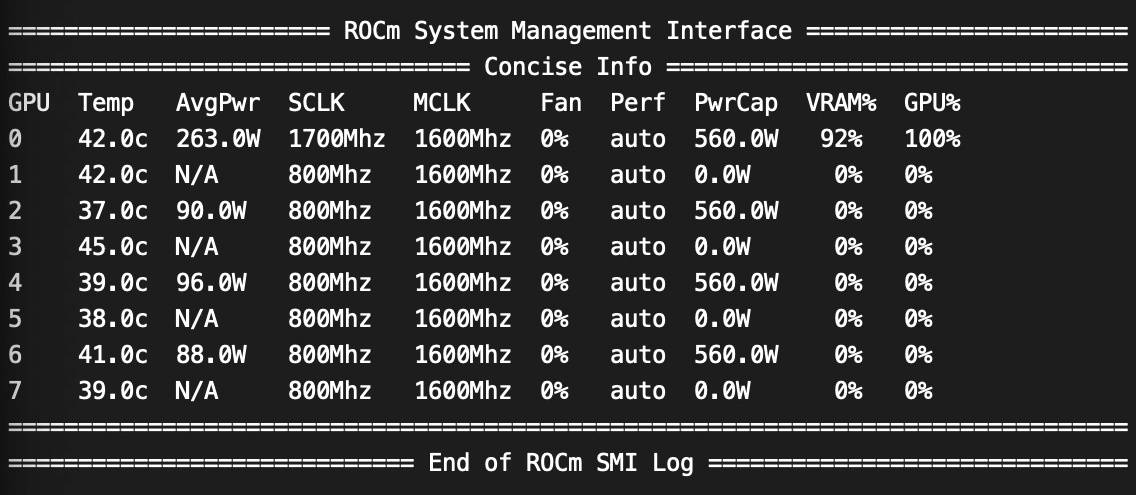
\includegraphics[width=\linewidth]{figures/threshold-vtkm-gpu-usage-crusher-small.png}
  \caption{
    ParaView, with integrated VTK-m accelerated filters, running on Crusher.
    VTK-m is using the Kokkos device adapter.
    The output of rocm-smi command is being used to verify and monitor GPU usage by the filters.
    \ken{I think it would be better to move this figure (or something like it) to the ParaView section.}
  }
  \label{fig:paraview-crusher}
\end{figure}

%\sujin{
%The first two paragraphs can be simplified by referring to the device adapter explanation in the VTK-m overview section
%}
As described in the overview of VTK-m,
one of the main features that VTK-m supports is ``write once, compile anywhere'' for its algorithms.
%VTK-m filter’s are implemented in modern C++. The build system of VTK-m can then compile these for one or more of the various parallel devices that it supports. This level of compatibility is achieved through the use of an abstraction layer in VTK-m called the \texttt{DeviceAdapter}.
A device portability layer called a device adapter allows algorithms written with standard C++ features run across all devices.
These device adapters wrap a parallel execution capable device and provide functionalities for parallel-task scheduling, memory management, and several commonly used parallel algorithms like sort, reduce, etc, through a common interface.
These are implemented on top of the native libraries used to program these devices.
%At the most basic level, a device adapter only needs to provide support for memory management on the device, a way to execute an n-way, fine-grained, parallel task on the device, and atomic operations.
%There are generic implementations for all of the parallel algorithms like sort, reduce, scan, etc, but it is possible to override these with specialized implementations for best performance.
%The early versions of VTK-m had \texttt{DeviceAdapter} implementations for single threaded CPUs using standard C++, multithreaded CPUs using the threading building blocks library or OpenMP, and GPGPUs using CUDA.

When the architectures for the initial two major Exascale machines, Aurora and Frontier, were announced, it was revealed that they would be using two completely new GPGPU architectures, with their own native libraries (SYCL and HIP).
This would have required additional two new device adapter backends.
Although the device adapter layer greatly simplifies the porting of VTK-m code, implementing device adapters themselves is not trivial.
So, although it would be technically feasible to design device adapters for two new devices, it would have required significant effort.
%Maintaining these backends together with the already existing backends was would require a lot of effort, especially for a project that is primarily concerned with implementing highly parallel visualization algorithms.

For these reasons, we looked towards another ECP project called Kokkos~\cite{Edwards2014, Trott2022}. Kokkos is a library for implementing performance portable applications in C++. Similar to VTK-m, Kokkos also supports multiple device backends, including HIP and SYCL used by the Exascale systems. So, with just one device adapter built on top of Kokkos, we are able to target both the machines.
This allows us to write the VTK-m device adapter once to the Kokkos API and defer the work of interfacing with the different ECP device APIs to the Kokkos team, who were already doing this for other ECP projects.

\ken{Is there anything more to be said about the interface? Was there anything particularly challenging? Any mismatch between the APIs? Any ``hacks'' that might have happened?}


\subsection{Addition and then Removal of Virtual Methods}
\label{sec:virtual-methods}

\assign{Ken}

Ideally, an algorithm
%that operates on arrays
will know the data types that it will operate on.
Unfortunately, this is seldom the case for VTK-m where data ingested from different sources can have any number of basic types
%(32- or 64-bit floats or fixed precision values encoded in integers)
and different types of memory layout.
In the early years of ECP, this problem was addressed by compiling algorithms in VTK-m for all possible types that could be encountered.
However, the amount of potential cases generated is too large to be practical.

C++ objects with virtual methods are a natural solution to this problem, and as they became available on CUDA devices, VTK-m started using virtual methods to hide the structure of arrays.
This originally addressed some of the issues with type abstraction.
However, this solution worked poorly and was later abandoned for two reasons.
First, using virtual methods introduced problems with library linking as the compilers had to collect any possible code that might be needed to be loaded on the device.
Second, when ECP announced that its Exascale machines would be using GPUs other than CUDA, it was unclear how well they would support virtual methods or even if they would be supported at all.

Consequently, the VTK-m development team pivoted.
Virtual methods were removed from the VTK-m code that ran on devices.
To manage the operations on types without using virtual methods, VTK-m employed a trio of strategies: multiplexing the type in the algorithm, generalizing the stride in arrays, and providing fallbacks when unexpected types were encountered.

The first strategy, multiplexing, required the use of a type agnostic storage object.
For this, a \texttt{Variant} class was added to VTK-m.
The \texttt{Variant} takes a list of types as template parameters, and it can hold exactly one of these objects at a time.
At runtime, the proper type can be queried and extracted.
%Implementing the \texttt{Variant} to avoid type punning across all device compilers was challenging.
Although multiplexing from a variant object still requires separate compilation for all possible types, it limits the code that must be recompiled to make it more manageable.

The second strategy required a redesign of the array management in VTK-m.
Where the original design of array management completely abstracted the implementation, the new design based array management on known buffers of memory.
This in turn provided a way to generalize the representation of an array component by defining a stride in the buffer.
In this way, an algorithm no longer had to be compiled for a specific data layout.
It could instead apply a stride to the array and use any layout.

The third strategy recognized that although a great number of types are possible, many are rarely if ever encountered in practice.
Therefore, instead of attempting to compile a function for any possible type, it is possible to instead compile for the most likely types and then have a fallback for the cases when the type is unexpected.
The typical solution is to copy the array of unknown type to an array of a known type.
This feature was included into the filter interface overhaul, which is described in the next section.

\subsection{Filter Interface Overhaul}

\assign{Ollie}

The majority of algorithms in VTK-m are contained in what is called a ``filter'' object.
A filter takes a data set, performs some operations to modify it, and returns the resulting data set.
Filters provide the outwardly facing API to processing data in VTK-m.
However, as previously described, these data sets can have any number of data types and structures.
The VTK-m filter base class needs to provide a mechanism to resolve data types.
That is, the filter base class needs a way to call a templated method in a derived implementation class with fully resolved data types.

Since a C++ template method can not also be a virtual function, which is needed for typical runtime polymorphism, the original design used a rather complicated technique called the curiously recurring template pattern (CRTP) \cite{Coplien1995} to emulate it.
CRTP works by making the type of the derived class a template argument to the base class.
When the base class needs to call a method in the derived class, rather than use a virtual method it recasts itself as the derived class and calls the method directly.
This allows the base class to iterate through a list of supported data types and call a templated method in the derived class to implement the algorithm on each one.

%The addition of \texttt{Variant} and the redesign of array management in VTK-m also enabled us to further redesign the developer's interface for \texttt{Filter}s.
%Previously, a filter implementation had to provide a \texttt{DoExecute} method that took a template \texttt{ArrayHandle<T>} as one of its arguments.
%Filter base classes would iterate through a list of supported data types, defined by the filter developer, instantiate and call \texttt{DoExecute} with each of the concrete type \texttt{T}.
%There were several downsides of this design.
%First, as mentioned above, we had to instantiate a large number of \textit{DoExecute}, one for each of \texttt{T} in the list.
%Second, since a C++ template method can not also be a virtual function which is needed for runtime polymorphism, the original design used a rather complicated technique called \emph{Couriously recurring template pattern (CRTP)} to emulate it.

However, using CRTP also made the base filter class itself a class template, and its execution methods required exposed definitions that needed to be recompiled at every instance of its use.
This made the VTK-m filter library essentially a header-only library, and clients using it had to include all the necessary implementation in the header files.
When compiling client code, all those header files had to be parsed and classes and methods had to be instantiated.
As a consequence, it took a long time to compile applications of VTK-m.
This issue was most prominent when compiling for GPU devices since most device compilers were not as efficient in handling C++ templates as host compilers.
When integrated as part of an in situ pipeline, simulation code calling VTK-m's filters also needed to be compiled by a device compiler, thus exacerbating the problem.
In some extreme cases, the whole compilation process took more than 24 hours to complete.

The new design turned this type dispatching mechanism around.
The responsibility of type dispatching was shifted from the filter base class to the derived implementation classes.
The execution method in the derived class is no longer a template; it accepts a data set containing ambiguous types.
This increases the burden on the algorithm developers who now have to resolve types themselves.
To compensate, VTK-m provides an alternate dispatching mechanism by providing various forms of a ``cast-and-call'' mechanism on the data set's elements.
The derived filter performs the type dispatching by passing a data set element to a cast-and-call along with a templated, callable object.
This callable object is generally the type dependent, core business logic of the filter implementation wrapped inside of a C++14 generic lambda expression.
The lambda expression will be instantiated with types from a pre-defined type list by the cast-and call mechanism.

The cast-and-call will attempt to resolve the data to a prescribed list of types.
When the type of the data is not part of the type list, the cast-and-call can fallback to a known type as described in the previous \nameref{sec:virtual-methods} section.
The pre-defined type list and fallback limit the number of instantiations of the lambda expression.
Using cast-and-call with lambda expressions in this way also limits the portion of code to be instantiated.
In contrast, the original design required the whole body of the filter implementation to be instantiated.

Since the filter execution methods are no longer template methods, they can be virtual methods.
Note that the filter methods in question are explicitly run in VTK-m's control environment, which means they will only be run on the CPU host of the machine.
Previously discussed issues with virtual methods on GPUs do not apply here, so creating virtual methods here is not problematic.
The virtual methods eliminate the need to use the CRTP technique.
As a consequence, the whole filter class hierarchy has became non-template classes as well.
The library is no longer a header-only library and can be built as a traditional, pre-compiled library.
The filter library is further divided into several modules with each separately compiled into a \texttt{.so} file.
Applications now do not need to be compiled by a device compiler simply because they are using VTK-m.

The ability to control template instantiation and separate, concurrent compilation of the filter library has greatly reduced application build time because they no longer has to compile many VTK-m templates.
Rather, applications simply link to methods in the VTK-m library.
We have also found that the new approach provides other compile-time saving opportunities within the library.
For example, some filters incorporate the functionality of others as a subprocess.
The new filter structure allows filters to be compiled once and have their functionality leveraged by other filters.
For example, the compilation of VTK-m's material interface reconstruction filter was reduced by a factor of 9 by linking to the mesh quality filter rather than recompiling it.
The new filter structure also enables dividing the code into multiple translation units (i.e. separate C++ source files).
Although this does not necessarily reduce the aggregate compile times, it more effectively leverages cores in parallel builds and reduces the possibility of compiler crashes from running out of resources.
%\ollie{Ken can you add some concrete timing measure as you did before here?}
%\ken{I will look. I probably don't have anything concrete. I'm not sure I captured enough data to measure the time before the filter change and the time after. (A lot changed in the interim anyway.) But I think I can pull up a couple of examples.}

\subsection{GPU-to-GPU Transfers}

Modern HPC GPUs allow direct GPU-to-GPU communication. This provides GPUs with an efficient mechanism to directly send data stored in their device memory to the target GPU device memory. This contrasts with the traditional and costly GPU communication pattern that consists in first copying the desired data from the device memory to host memory, transferring it, and then again copying the received data from host memory to device memory.

Enabling this feature in VTK-m required changes in the source code of both VTK-m itself and DIY, a third-party library that VTK-m uses to manage its MPI communication~\cite{Peterka2011,Morozov2016}.
%The reason for making changes to DIY is that VTK-m delegates data marshaling and remote communication through the DIY library.

The DIY library changes consisted of adding routines that allow sending and receiving raw pointers directly encapsulated in a newly introduced ``blob'' data type. This contrasts with the regular operation of DIY that copies and serializes data before sending and receiving. In addition to that, we have also introduced a new API in DIY that controls the ownership of the passed raw pointer.

The corresponding VTK-m changes consisted of modifying the VTK-m class that manages memory buffers and their location among host and devices.
In particular, the changes overwrite the DIY serialization to directly pass these memory buffers to and from DIY.
Additionally, a new CMake option named \texttt{VTKm\_ENABLE\_GPU\_MPI} that activates direct GPU-to-GPU communication of VTK-m buffer objects was added.
This in turn, enables direct GPU communication in VTK-m since most of the VTK-m storage entities are composed of VTK-m buffers. 

The main challenge found during the implementation of this feature was maintaining compatibility with the Frontier target system.
The problem was that the software stack in the target system was a moving target with frequent updates that in many cases required us to modify build and runtime parameters and, in some other cases, perform changes to the VTK-m and DIY source code.
This challenge was minimized by provisioning the VTK-m Gitlab project with nightly jobs that build and run tests using this feature in the Frontier test-bed system.
This allowed us to quickly identify problems arising in changes to either VTK-m's source code or the Frontier software stack.
